\chapter{Planning}
\label{chap:Planning}

\section{Project Plan}
\label{sec:PlanningProjPlan}

The Project plan gives an overview of our plans for the project. It includes time estimates, group organization, risk management, and quality assurance.

\paragraph{} Figure \ref{fig:PlanningProjPlanGantt} shows the project plan that was made during the planning phase, and gives an overview of the main phases of the project. Each phase also has its own assignments, that are mentioned in each phase's chapter in the report.

\paragraph{} When the group started implementation, some changes were made to the project plan to make room for changes in the design. Work on the report began at the same time as system development, and, more or less, continued throughout the project.

\paragraph{} The plan is divided into days and weeks of work, and each phase is given a slice of this time. The active time of the project is a total of 12 weeks, since time at the beginning was spent on the kick-off of the project. At the end, there is a delivery and presentation of the project.

\afterpage{
\clearpage
\begin{landscape}
    \centering
    \begin{figure}
        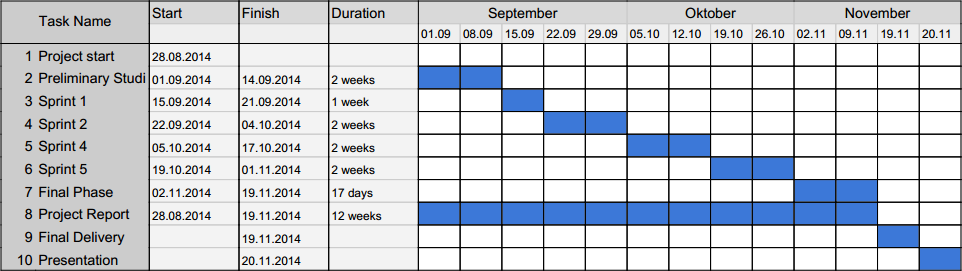
\includegraphics[width=\linewidth]{./Planning/img/GANT}
        \caption{Gantt diagram for the project.}
        \label{fig:PlanningProjPlanGantt}
    \end{figure}
\end{landscape}
}

\section{Methodology}
\label{sec:PlanningMethod}
During the preliminary studies, two development processes were considered, the Waterfall model and the Scrum model. As a result of the preliminary studies the Scrum model was chosen. This section deals with a short justification of why Scrum was the best choice, and how we adjusted the process to fit this project.

\subsection*{Scrum, Our Choice in Methodology}
\label{subsec:PlanningMethodChoice}
At the beginning of this project, the customer presented their vision, but did not present us with any concrete requirements for the final product. As a result of this, it was important to choose a development process where requirements can be changed and extended easily. For this, Scrum was the best fit. Another reason for choosing Scrum was the needed involvement of end users for feedback. This also required us to be able to adapt to change, as feedback often leads to changes to the requirements. Being a project with very few initial requirements it was important to involve end users as early as possible, and present a  product iteration as often as possible to the customer. With these two requirements for the project, Scrum was the best choice. A detailed description of Scrum in comparison with the Waterfall model is termed in section \ref{sec:PrelimMethod}.

\subsection*{Required Adjustments}
\label{subsec:PlanningMethodAdjust}
Certain aspects of the Scrum methodology did not fit the project team. Because of this, adjustments to the method had to be made. Due to other courses and assignments, it was not feasible for the team to meet every day, and we had to reduce the daily stand up meetings to biweekly meetings. Team members were responsible for reporting their work status to the Scrum master. That way the work progress could be tracked outside of meetings. Our Scrum team created a product backlog and at the start of each sprint selected which of the requirements should be fulfilled by the end of that sprint.

%TODO CHECK PHRASING
\paragraph{} In contrast to traditional Scrum, we had sprints with the duration of only one week in the beginning of the project. That way it was easier to manage the sprint, when no team members had prior experience working with Scrum. After the first few weeks the sprint duration was extended to approximately two weeks.

%TODO CHECK PHRASING
\paragraph{} At the end of each sprint we had a sprint delivery where we presented the product to the customer. This made it possible for the customer to see the progress of the project, and their frequent feedback gave us the ability to ensure that the project was headed in the right direction by finding problems early. The retrospective meeting after each sprint was helpful to get an overview over potential problems during the last sprint and what we could do to improve the work process for the next sprint. 

%TODO CHECK PHRASING
\paragraph{} The project work was divided into two groups. The first group would focus on implementation and the second group on the report. To track which people were working on what tasks, we used the Issue Tracker Tool YouTrack. This tool helped us assign tasks to team members and set the status of tasks. All team members could see what the others were working on and when they were finished. It also gave us an integrated burndown chart, which shows the work left versus the time left.


\section{Group Organization and Project Management}
\label{sec:PlanningGroupOrg}
Our group consists of seven people, and most of them have more than one role within the team. There are three main roles in a Scrum team; product owner, Scrum master and Scrum team. The overall structure of this group is flat, since the group is fairly small.

\subsection{Roles}
\label{subsec:PlanningGroupOrgRoles}
\paragraph{The Project Lead/Scrum Master} is responsible for the overall progress of the project and organizational tasks such as planning and workload. The project lead has to make plans for sprints, meetings and deliveries and maintain contact with the customer and supervisor.

\paragraph{Team}
\begin{itemize}
    \item \textbf{The Implementation Lead} has  final responsibility over the system. He is responsible for keeping track of what needs to be done on the system to make it ready for delivery. He also has a responsibility to be available to help other with any problems they might have regarding the implementation.
    \item \textbf{The Requirements Specialist} initial responsibility is making sure a system requirements document is created and important use cases are ready. They also have a responsibility to make sure the final system fulfills these requirements.
    \item \textbf{The Document Managers} are responsible for the work done on the report. They are responsible for assigning sections that need to be written in the document and making sure the different parts match each other.
    \item \textbf{The Test Managers} work closely with the requirements specialist to make tests for the final system test, as well as doing tests while development is ongoing. They are responsible for making a test plan and making sure the plan is executed in the final stages of the project.
    \item \textbf{Developers} are responsible for creating quality code for any task they may be assigned to, and keeping the repository up to date with their code. They also have to make sure to keep the time spent up to date on our backlog, and to take responsibility for any open issues they are able to solve.
    \item \textbf{Architects and designers} are responsible for the overarching design and higher level system architecture. As with developers, they have to make sure to keep their time tracking up to date, and to be ready to take care of any issues.
\end{itemize}

\subsection{Allocation of Roles}
\label{subsec:PlanningGroupOrgAllocation}
Each member of our team has at least one role with its accompanying responsibilities. We selected these based on the needs of the project and the wishes of the group. In addition to any roles allocated here, all group members are expected to be able to jump in and do a critical task as needed, and the Project Lead is responsible for keeping track and allocating these tasks. We tried to limit the number of roles, since the group is fairly small.

\begin{minipage}{\linewidth}
\centering
%\setlength{\tabcolsep}{22pt}
\rowcolors{1}{blue!20}{blue!10}
\begin{tabular}{|l l|}
    \hline
    \textbf{Project Lead} & \begin{tabular}{l}
                            Jonas F. Therkelsen \\
\end{tabular} \\
    \textbf{Implementation Lead} & \begin{tabular}{l}
                                   Valerij Fredriksen \\
\end{tabular} \\
    \textbf{Requirements Specialists} & \begin{tabular}{l}
                                        Brage E. Jahren \\
\end{tabular} \\
    \textbf{Developers} & \begin{tabular}{l}
                 Yngve Bloch-Hoell \\
                 Valerij Fredriksen \\
                 Brage E. Jahren \\
                 Hans Olav Slotte \\
                 Manasa Vallamkondu \\
    \end{tabular} \\
    \textbf{Document Manager} & \begin{tabular}{l}
                                Julia Schneider \\
    \end{tabular} \\
    \textbf{Architects and Designers} & \begin{tabular}{l}
                               Brage E. Jahren \\
                               Valerij Fredriksen \\
                               Jonas F. Therkelsen \\
    
    \end{tabular} \\
    \hline
\end{tabular}
\end{minipage}

%TODO ONE PASS DONE RECHECK
\section{Project Phases}
\label{sec:PlanningProjPhases}
The team divided the project into seven different phases. these consist of the preliminary studies, five sprints and a final phase with documentation and delivery. The preliminary studies includes brainstorming and development of the idea, rough designs and mockups made in dialog with the customer. Following the preliminary studies were the sprints. Each sprint was between one and two weeks long, focusing on implementing the system, group dynamics, and contact with the supervisor and the customer. The final phase of the project consists of documentation and delivery of the report and product. No new features to be developed during this phase, but the system is tested to be fully functional and ready for delivery.

\subsection{Preliminary Studies}
\label{subsec:PlanningProjPhasesPrelim}
The preliminary studies took place during the first two weeks of the project. At our initial meeting with the customer, the project team was presented with the customer's vision of a digital product. Over the next two weeks, the team met on almost a daily basis developing the concept for a product based on the vision presented by the customer. When the concept was approved, different roles were assigned to the members of the group, and technlogy platforms and frameworks decided upon and basic implementation started. We also made some initial assessments of the different development methodologies during this phase, but no final conclusion was made about whether to choose Scrum or the Waterfall method.

\subsection{Sprints}
\label{subsec:PlanningProjPhasesSprints}
The Sprints of the project comprised the next eight weeks of the project. There were four separate sprints, most of which were two week long sprints. The main focus of the sprints was system development and creating first drafts of the relevant sections of the report. Each sprint has its own corresponding chapter, \ref{chap:S1} through \ref{chap:S5}, where the efforts of each sprint are described in depth.

\subsection{Documentation and Delivery}
\label{subsec:PlanningProjPhasesDocDel}

This phase consisted of the last two weeks of the project. This is the phase when all the work done during the semester will be given their final shape. No new features were implemented, but bugs were fixed after testing, and the system was given the final layer of polish before delivery. Much of the group also worked on making the report as good as possible, and writing necessary chapters, especially concerning further work to be done. Towards the end, everyone was working on proofreading or preparing for the presentation.

\section{Risk Management}
\label{sec:PlanningRiskMan}
We will now focus on the risk management of the project. The whole project will be analysed and risks are grouped by the following criteria:
\begin{itemize}
\item \textbf{A} Group communication
\item \textbf{B} Issues with the customer
\item \textbf{C} Risks in relation to planning
\end{itemize}
%TODO CHECK PHRASING
Once each risk has been placed into a category, the first letter of its ID has been determined. All risks in a category are then numbered to give them their final ID. Once risks have been decided, we moved on to deciding their probabilities and consequences in order to evaluate how problematic they would be for the project. The following table shows the meaning of each of the consequence levels.

\begin{minipage}{\linewidth}
\setlength{\tabcolsep}{10pt}
\centering
\rowcolors{1}{blue!20}{blue!10}
\begin{tabular}{ |l|p{5cm}| }
	\hline
	\multicolumn{2}{|c|}{\cellcolor{gray!25} Consequence Levels} \\
	\hline
	High & This risk is a major problem. It has a big impact on the project, especially on finishing the project in the given time.\\
	Medium & This risk is big, but still manageable. Mostly this leads to more work for the team members. \\
	Low & Risks with a minor impact on the project. \\
	\hline
\end{tabular}
%Caption here
\captionof{table}{Description of consequence levels. \label{tab:PlanningRiskManRiskLvl}} 
\end{minipage}

In order to evaluate the probability of a risk happening, the group members' experience was important. Each member of the group ranked the risks according to what they thought the chance of a risk happening was (high or low). A clear majority determined the result, and an unclear majority or tie resulted in a medium probability.


When we had determined both these values for the risks, we could calculate their risk levels. The risk level is found using the following formula.
\begin{equation}
R_L = C_L \cdot p
\end{equation}
Where \( R_L \) is risk level, \( C_L \) is consequence level, and \( p \) is probability. For \( C_L \) and \( p \) high is counted as \( 1 \), medium as \( 0.5 \), and low as \( 0 \). With this formula \( R_L \) will have one of four values \( (1, 0.5, 0.25, 0) \). The matrix in table \ref{tab:PlanningRiskManRiskMatrix} shows the different risk levels resulting from this formula.

\begin{minipage}{\linewidth}
\centering
\begin{tabular}{cc|c|c|c| }
  \cline{3-5}
  & & \multicolumn{3}{|c|}{Consequence Levels} \\ \cline{3-5}
  & & High & Medium & Low \\ \hline
  \multicolumn{1}{|c}{\multirow{3}{*}{Prob.}} & \multicolumn{1}{|c|}{High} & \cellcolor{red!30} High & \cellcolor{red!30} Medium & \cellcolor{green!15} Low \\ \cline{2-5}
  \multicolumn{1}{|c}{} & \multicolumn{1}{|c|}{Medium} & \cellcolor{red!30} Medium & \cellcolor{green!15} Medium-Low & \cellcolor{green!15} Low \\ \cline{2-5}
  \multicolumn{1}{|c}{} & \multicolumn{1}{|c|}{Low} & \cellcolor{green!15} Low & \cellcolor{green!15} Low & \cellcolor{green!15} Low \\ \cline{2-5}
  \hline
\end{tabular}
\captionof{table}{Different risk levels. \label{tab:PlanningRiskManRiskMatrix}} 
\end{minipage}

The matrix displays if there is demand for action (red) to develop a proactive and reactive strategy. If the colour is green the probability or consequence level is low, or both are medium, and we decded that there was no need to develop a strategy against it. Figure \ref{fig:PlanningRiskManRisks} displays the risks we considered and their consequence and probability levels. In addition there is a short explanation for why these levels were chosen.

\paragraph{}After we had evaluated the risks and found out which risk level each of them belonged to, the next step was to find strategies to cope with those risks that were given a red risk level. Table \ref{tab:PlanningRiskManCriticalRisks} displays the critical risks and the proactive strategies created to prevent them. In adition there are also reactive strategies to cope with risks that cannot necessarily be prevented, such as illness.
%
\rowcolors{1}{blue!20}{blue!10}
\begin{tabular}{|p{0.07\linewidth}|p{0.18\linewidth}|p{0.7\linewidth}|}
    \cellcolor{gray!25} \textbf{ID} & \cellcolor{gray!25} \textbf{Risk} & \cellcolor{gray!25} \textbf{Strategy} \\
    \hline
    A2 & Failure to reach customer expectations. & 
      \begin{itemize}
        \item Use Scrum to get frequent customer feedback through an iterative approach.
        \item Customer meetings once per week to show results.
      \end{itemize} \\
    C1 & Illness or group member absence. &
      \begin{itemize}
        \item Absence:
          \begin{itemize}
            \item Early notice about absence.
            \item Tasks assigned at the beginning of the week to give everyone the ability to spend time when it is available.
          \end{itemize}
        \item Illness:
          \begin{itemize}
            \item Inform the group about illness as immediately.
            \item Assign critical tasks to other people.
          \end{itemize}
      \end{itemize} \\
    C2 & Bad division of workload. &
      \begin{itemize}
        \item Divide the team into two groups, each focusing on either the report or the implementation.
      \end{itemize} \\
    C4 & Underestimation of workload/wrong prioritization &
      \begin{itemize}
        \item Meet twice a week with status updates on assigned tasks
        \item Make estimations as a team rather than indivituals.
      \end{itemize}
\end{tabular}
\captionof{table}{Critical risks and risk management strategies. \label{tab:PlanningRiskManCriticalRisks}}

\afterpage{
\clearpage
\begin{landscape}
    \centering
    \begin{figure}
        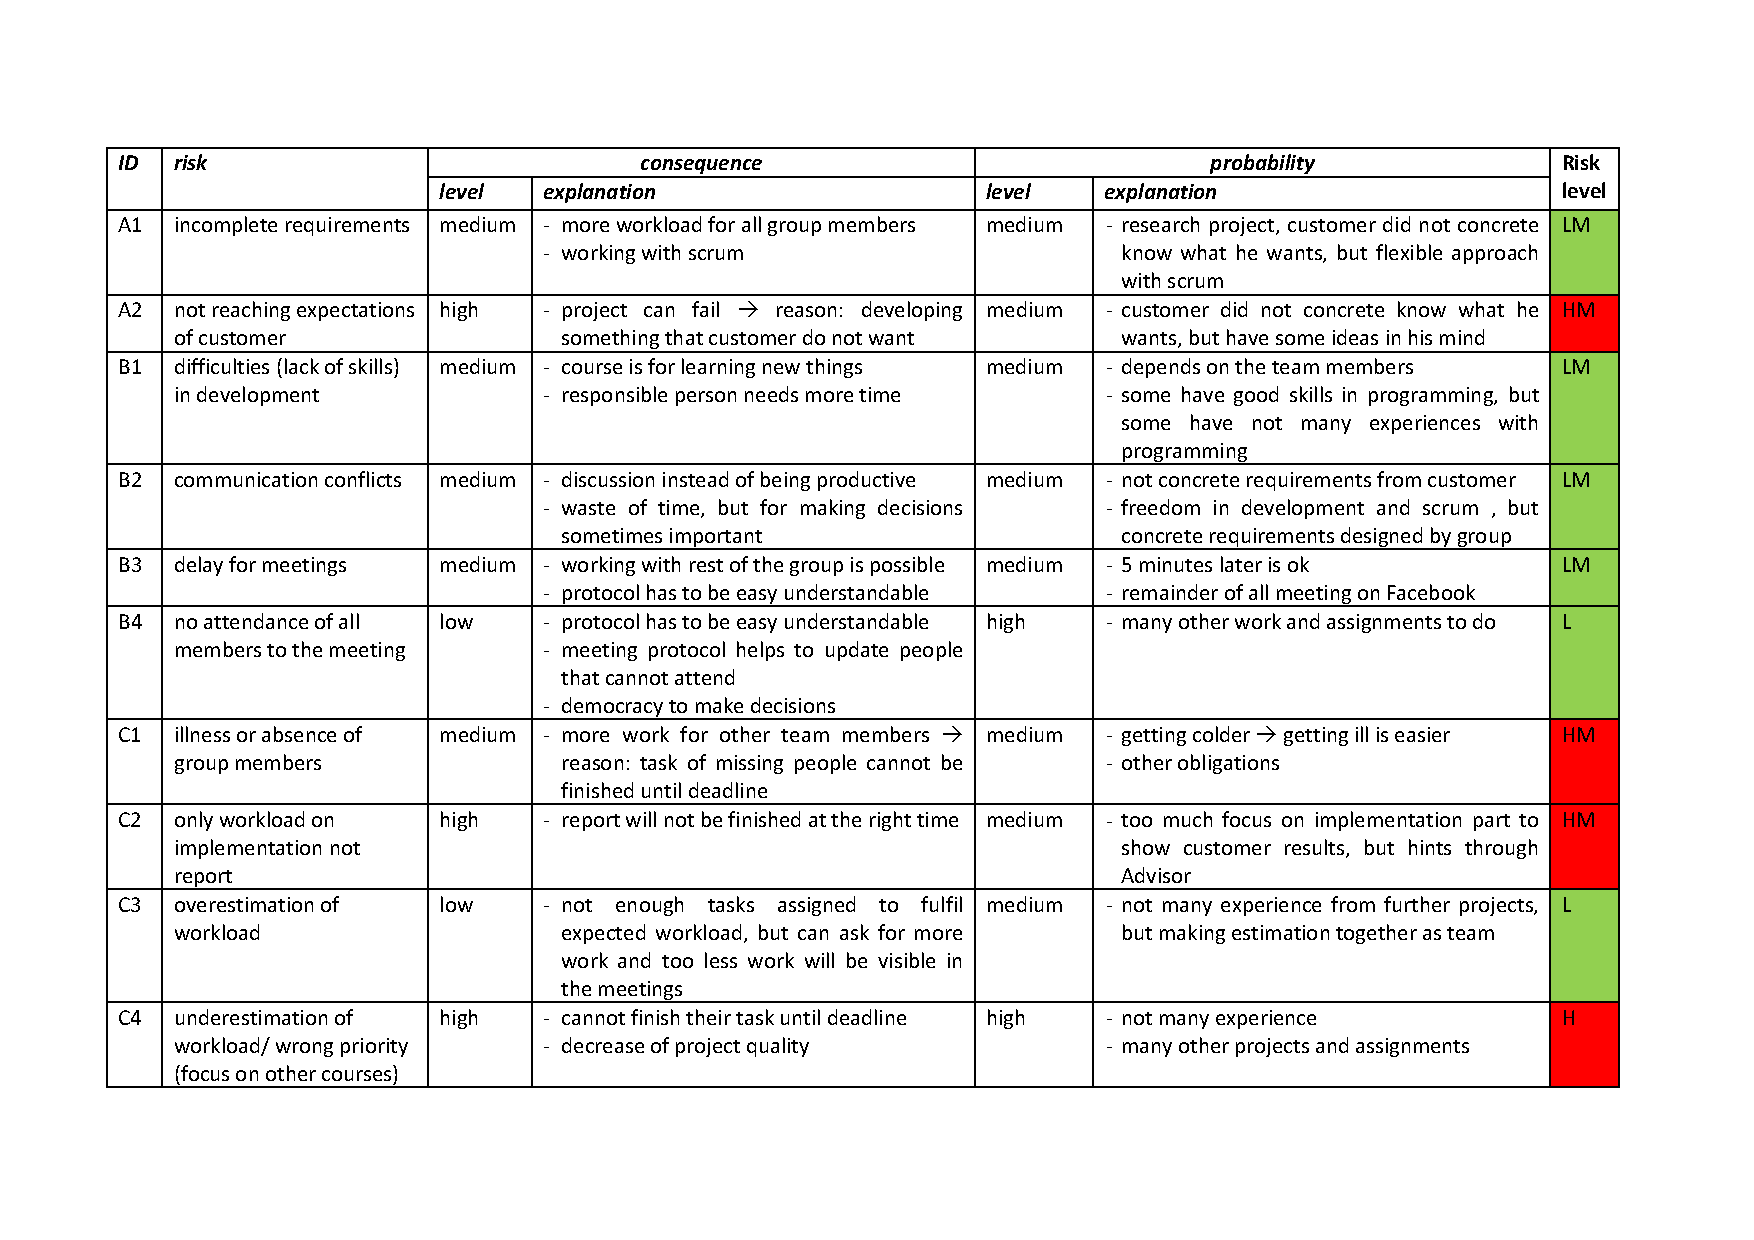
\includegraphics[width=\linewidth]{./Planning/img/Risk.pdf}
        \caption{Risks for the Alternative Spaces project.}
        \label{fig:PlanningRiskManRisks}
    \end{figure}
\end{landscape}
}

\section{Quality Assurance}
\label{sec:PlanningQuality}
%TODO RECHECK PHRASING
In order to ensure a high quality in the final project, the process, and all documents related to it, we needed to establish a set of routines. These routines were divided into two main categories. Internal and external routines. The internal routines include everything that concerns the progress of the project, such as revision control and other tools. It also includes standards for documents and communication, both during and outside of meetings. Exteral routines involves all rules concerning and agreements with the customer and the supervisor.

\subsection{Internal Routines and Intrateam Communications}
\label{subsec:PlanningQualityRoutines}
%TODO RECHECK PHRASING
Every member of the team had many liabilities outside this project. This included assignments in other courses, or working on the side of their studies. To achieve the projects goals it was important to make it as flexible as possible. As long as everyone did what was expected, every member could decide when during the week assigned tasks would be finished. To ensure that the work was being done, some tools were used to display each member's progress. These were a work sheet on Google Drive, as well as the project management tool YouTrack. The work sheet was used to record the amount of time spent by everyone on the project, while YouTrack was used to assign tasks and have an overview of their progress. Every task was given en estimated time and as people finished tasks, they reported actual time spent.

\begin{figure}[ht!]
\centering

\includegraphics[width=90mm]{./Planning/img/YouTrack_logo}
\caption{YouTrack \label{fig:PlanningQualityRoutinesYouTrack}}
\end{figure}

\paragraph{} Finding regular meeting days that fit into all team members' schedule was a challenge. In the end we managed to schedule meetings twice a week. The first meeting was to assign tasks, while the second was to prepare for the weekly meeting with the group's supervisor. Additional meetings were agreed upon through a Facebook group when necessary. Using Facebook was also usefol for asking questions when something was unclear or to bring up problems between meetings. The team also decided to choose a room where people could sit down and work together everyday, in order to increase motivation, and make it possible for anyone to show up and ask for help with any problems they might have encountered. As mentioned in section \ref{sec:PlanningRiskMan}, the group was divided into two focus groups, both to avoid focusing too much on one part of the project and to make sure the final product was better. Since the group had varying levels of experience working with web development, these groups were very beneficial to product progress.

\paragraph{} In each meeting each member of the group answered the following questions:
\begin{itemize}
  \item What have you done since last time?
  \item What problems or challenges did you face?
  \item What will you be doing until next time?
  \item Do you have any questions or something you want to discuss?
\end{itemize}
This helped the group and the project manager to get a clear overview of the project and it made the project progress transparent.

\subsection{Documentation Templates}
\label{subsec:PlanningQualityDocu}
To avoid forgetting information from discussions in group, customer or supervisor meetings, writing meeting notes were necessary. For each meeting protocol, the team used the structure displayed in \ref{fig:PlanningQualityDocuMeeting} to give the meeting documents a consistent layout.

\begin{figure}[ht!]
\centering

\includegraphics[width=90mm]{./img/Placehoder}
\caption{Meeting document template. \label{fig:PlanningQualityDocuMeeting}}
\end{figure}

\paragraph{} To organize all of the produced documents, the group used a Google Drive folder. This was used to store all parts of the report, meeting notes and other documents relevant to the project. The development focus group used GitHub to document changes in the source code. Figure \ref{fig:PlanningQualityDocuDrive} shows the structure of the Google drive folder.

\begin{figure}[ht!]
\centering

\includegraphics[width=90mm]{./img/Placehoder}
\caption{Meeting document template. \label{fig:PlanningQualityDocuDrive}}
\end{figure}

\paragraph{} The "E-mails" folder contains all mails to and from the customer. "General information contains all details about the project itself, for example the project compendium. In the "Meetings" folder all notes taken during group, customer and supervisor meetings were stored. To specify further, each file name contains the meeting type followed by the date, for example "Group - 15.09.14". This makes it easy to search through the documentation. The "Presentation" folder contains all presentations the group created for the customer or supervisor during the project. All documents belonging to the managing of the project were placed in the "Project management and Scrum" folder. For the documentation focus group, the most important folder was the "Report" folder. As seen in figure \ref{fig:PlanningQualityDocuDrive}, the folder contains a folder for each part of the report.

\subsection{Revision Control}
\label{subsec:PlanningQualityRev}
%TODO RECHECK PHRASING
The development group decided use Git and GitHub to monitor their progress. This made it possible for multiple members of the group to work on the source code at the same time. 
Using different branches for different functionality gave each member the chance have their own version of the source code. With this approach overwriting or other conflicts could be avoided. Every developer was responsible for making sure each commit was accompanied by a meaningful comment about changes made in that commit, and the Technical Lead was responsible for making sure the feature branch was tested before merging it with the master branch. If the feature branch was correct, the Technical Lead merged the branches and deleted the feature branch.

\subsection{External Routines and Customer Communication.}
\label{subsec:PlanningQualityExternal}
%TODO RECHECK PHRASING
Since the Work Research Institute is located in Oslo, most of our communication with the customer took place via Skype and e-mail. To simplify our communication with the customer, one team member was responsible for all contact with them. The meetings took place after each sprint, or when there were something we needed an answer to. The customer was informed of such meetings at least 24 hours ahead. As well as stating the time and date of the meeting, we also gave the customer an overview of the topics we wanted to discuss. At all of the customer meetings we made sure to get answers to the following questions:
\begin{itemize}
\item What are your thoughts on the status of the project right now and the progress so far?
\item Are you satisfied with our work so far? Are the results as expected?
\item Is there something we can do better or need to change?
\item What are the most important features you want us to implement during the next sprint?
\item Do you have any questions?
\end{itemize}
If the customer was unable to answer the questions during the meetings, the answers were sent by e-mail within 48 hours after the meeting. All e-mails from the customer were written in English and sent to all members of the team. If we had any questions to the customer outside of meetings, our customer contact would send the questions by e-mail. That way we ensured that the customer would not receive the same questions multiple times.

\subsection{Communication with the Supervisor}
\label{subsec:PlanningQualityAdvisor}
Each thursday during the project we had a meeting with our supervisor. At these meetings we presented the project status in order for the supervisor to get some insight into our progress and work process. The supervisor would point out problems we had not found ourselves, and also gave us input on what we needed to consider. To prepare for the supervisor meeting the group usually met on wednesday or thursday morning. In these meetings the team decided on what to present to the supervisor and updated all documents, worksheets and YouTrack. Links to all relevant documents on Google Drive were sent to the supervisor in advance, so that he could prepare for the meeting. During the meetings one member wrote notes, while the project manager chaired the meeting. The supervisor had access to all documents on Google drive at all times. This made it possible for the supervisor to follow the progress of the project, read the documentation and give hints or improvement suggestions.

\section{Software Development}
\label{sec:PlanningSoftwareDev}

In this section we will give an overview of the tools required for develoment and environment setup.

\subsection{Git and GitHub}
\label{subsec:PlanningSoftwareDevGit}

When working together in a group on shared code, having an efficient workflow requires having the ability to work on the common codebase simultaneously. This means having using some form of revision control software that can merge code automatically, or at least point to where manual merging is required. Some of the most popular of these today are Git, Subversion, and Mercurial. All of these could fulfill the needs of the project, but because we were most familiar with Git, and the Technical lead payed for private repositories on the GitHub servers, we chose to use Git and GitHub for our revision control.

\begin{figure}[ht!]
  \centering
  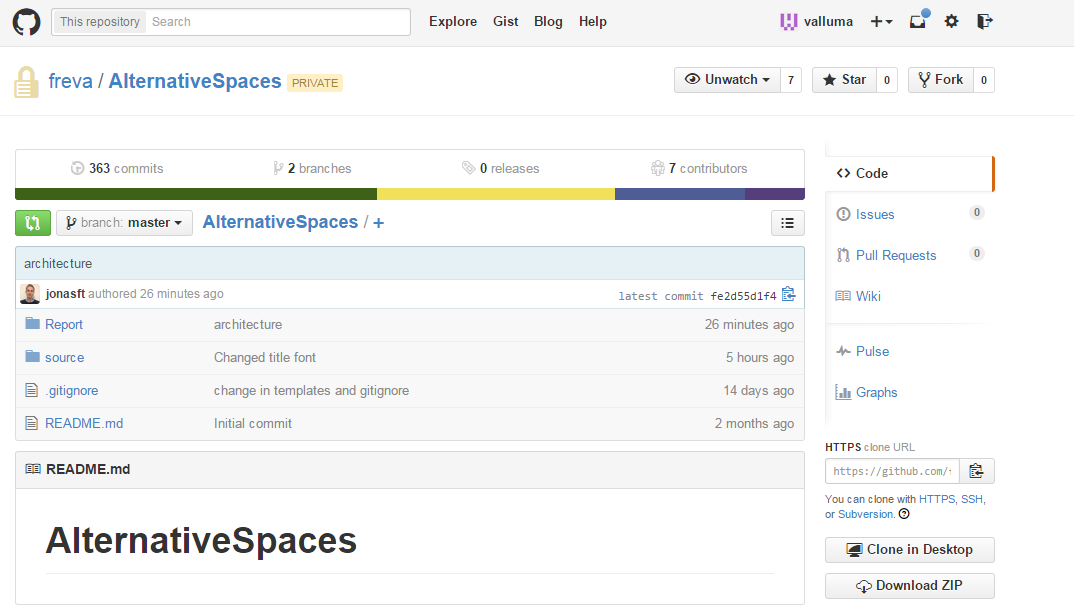
\includegraphics[width=\linewidth]{./Planning/img/ASpacesRepo}
  \caption{The Alternative Spaces repository on GitHub}
  \label{fig:PlanningSoftwareDevGitRepo}
\end{figure}

\subsection{Google Drive}
\label{subsec:PlanningSoftwareDevDrive}

Over the course of a project lasting 12 weeks, there are a lot of documents to write, both as part of the final report, and to keep track of activities within the group. Cooperative text editing software helps a lot in keeping communal documents available for everyone to view and work on. Google Drive, with its Docs feature, was ideal for our needs, since it was simple to use, and let everyone work at the same time. All members were also familiar with it, which made this choice very easy to make. The only significant drawback for our use of Google Drive is its sluggishness when working in large documents. This was alleviated by creating a larger amount of smaller documents, and keeping the Drive folders well organized.

\begin{figure}[ht!]
  \centering
  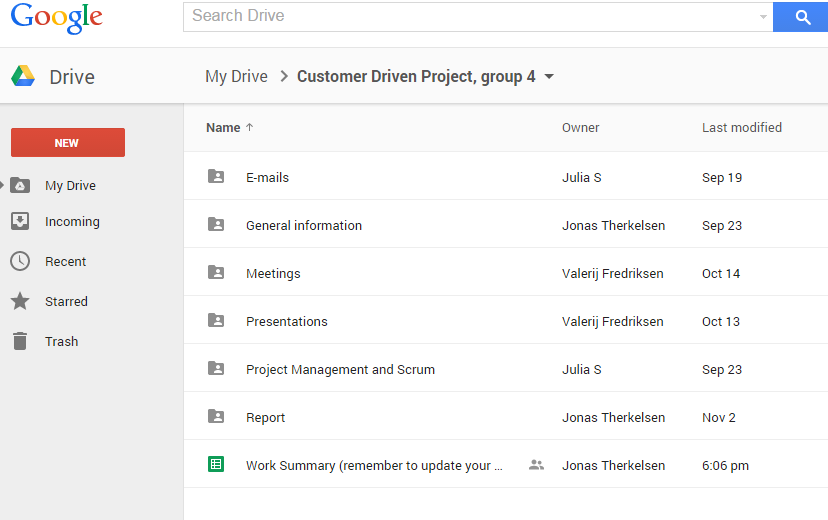
\includegraphics[width=\linewidth]{./Planning/img/Drive}
  \caption{The shared Google Drive folder}
  \label{fig:PlanningSoftwareDevDriveFolder}
\end{figure}

\subsection{Skype}
\label{subsec:PlanningSoftwareDevSkype}
Skype is a free software product owned by Microsoft, enabling registered users to have a simultaneous multi-way transfer of video and audio over the internet. These features allows users to have video calls for free over any distance. Skype also provides additional features like sharing files, messaging, and live screen sharing. The video, audio, and screen sharing capabilities of the service were used by the team in Trondheim when communicating with the customer in Oslo.

\subsection{IntelliJ IDEA}
\label{subsec:PlanningSoftwareDevIntelliJ}

In this group, few people other than the Technical Lead had a lot of experience with web development, and we decided that to help everyone more quickly set up their development environment we should all use the same integrated development environment (IDE). To make it even simpler, we decided to use the IDE the Technical Lead was most familiar with for this kind of work. He decided on IntelliJ IDEA, since it had integrated support for Git and GitHub, and would let people interface with the repo with a single click within the IDE. When we later decided on developing an Android application, we were also lucky in finding that Google had developed Android Studio, an IDE made for Android development, based on IntelliJ IDEA.

\begin{figure}[ht!]
  \centering
  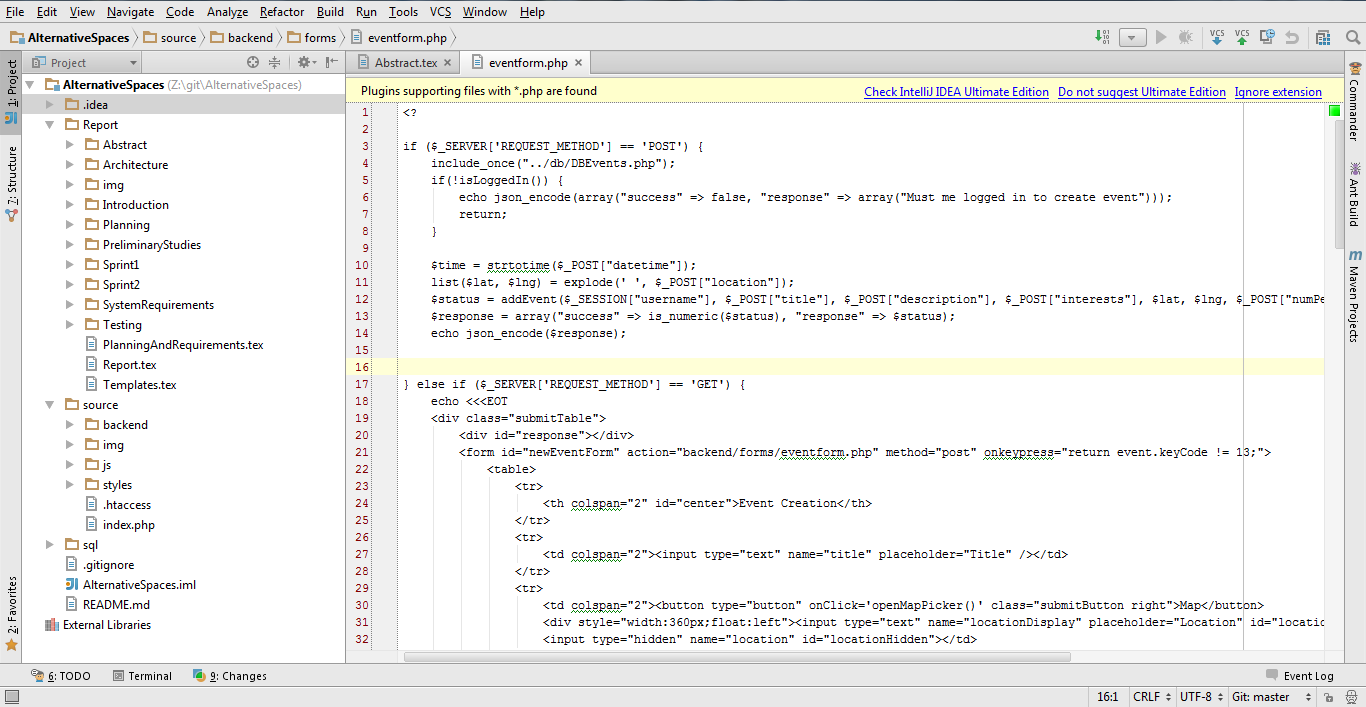
\includegraphics[width=\linewidth]{./Planning/img/IntelliJ}
  \caption{Standard project structure and view in IntelliJ IDEA.}
  \label{fig:PlanningSoftwareDevIntelliJView}
\end{figure}

\subsection{Android}
\label{subsec:PlanningSoftwareDevAndroid}

Android is a Linux-based operating system for mobiles and other small devices, mainly with touchscreens. As of 2013, it is the highest selling mobile operating system in the world overall, selling more than the rest combined. When we eventually decided to develop a small mobile app, the choice of which mobile was rather easy, since most of us owned Android devices, and those in the group who had experience developing mobile applications had done so on Android.

\paragraph{} Development is done in Java, which everyone in the group knows, and development can be done on any computer. However, the high number of different devices running Android, makes testing the application challenging, and since we only had our phones available, there is no guarantee that the app will work on all devices.

\begin{figure}[ht!]
  \centering
  
\includegraphics[width=40mm]{./Planning/img/AndroidLogo}
  \caption{Android.}
  \label{fig:PlanningSoftwareDevAndroid}
\end{figure}


\subsection{Languages}
\label{subsec:PlanningSoftwareDevLanguages}

\subsubsection{PHP} PHP is a widely used server-side scripting language for web development. Its syntax is similar to C and Perl, and is a dynamic, weakly typed, interpreted language. In our program, it us used for the back-end, including communication with the database, and getting the required forms for input.

\subsubsection{HTML} HTML is a markup language for creating web pages, which can be displayed by any common web browser. It is used to structure information. In ASpaces it has been used for front-end development along with CSS (Cascading style sheets) for describing the look and formatting of the site.

\subsubsection{JavaScript} JavaScript is a dynamic web-development language with a syntax similar to Java. It is used by browsers to allow client-side scripts to interface with the user, control the browser, communicate, and alter the content that is displayed. In our program it is used to make the website design more polished, by handling the front-end for comments and the 2D search.

\subsubsection{LaTeX} LaTeX is a document preparation and typesetting language based on the older TeX. It is widely used in academia, because it has large amounts of support for domain specific symbols and expressions found in many different disciplines. LaTeX was used for writing this document.

\subsection{PuTTY} 
\label{subsec:PlanningSoftwareDevPutty}

PuTTY is a terminal emulator, serial console and network file transfer program. It supports several network protocols, and can also connect to serial ports. We used the program to create and maintain the database for the site.

\begin{figure}
  \centering
  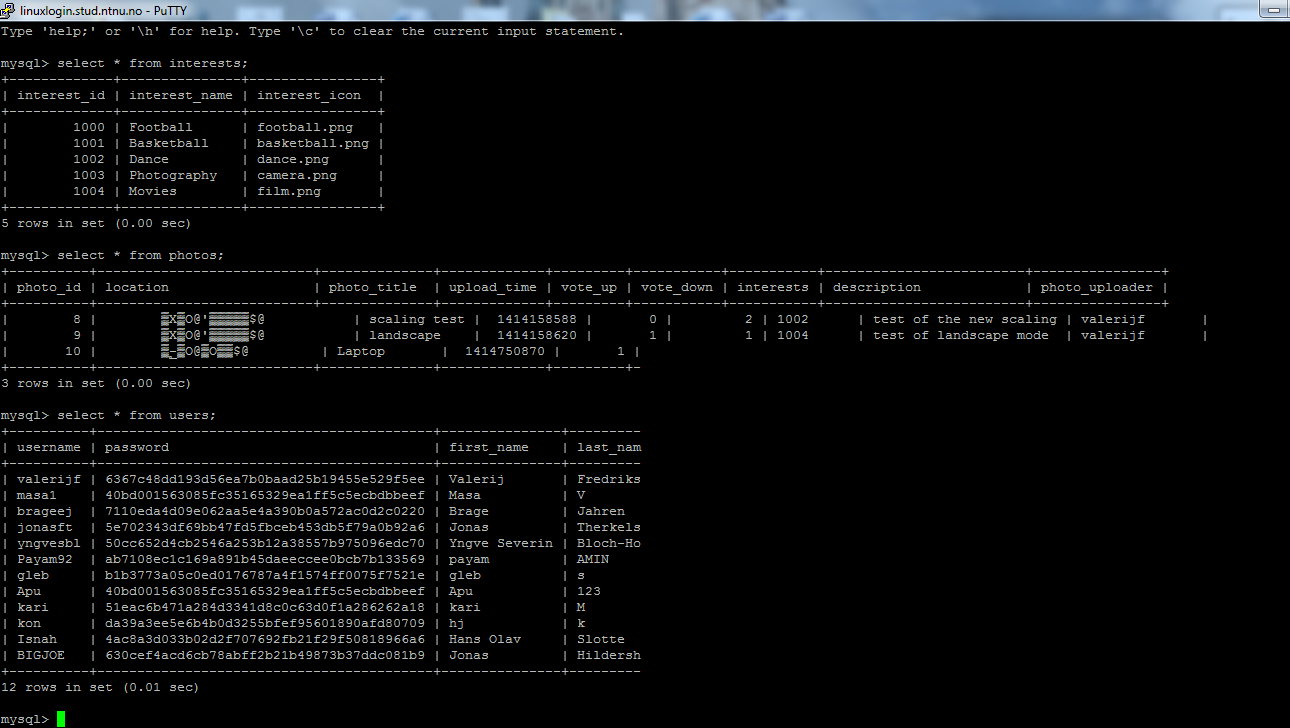
\includegraphics[width=\linewidth]{./Planning/img/puttydb}
  \caption{Database created and maintained in PuTTY.}
  \label{fig:PlanningSoftwareDevPutty}
\end{figure}

\subsection{YouTrack}
\label{subsec:PlanningSoftwareDevYouTrack}
YouTrack is a browser-based issue tracking system and project management software made by the same group that made IntelliJ IDEA, JetBrains. We used it mainly for its issue tracking, in order to assign tasks to team members and comment on issues easily.

\begin{figure}[ht!]
  \centering
  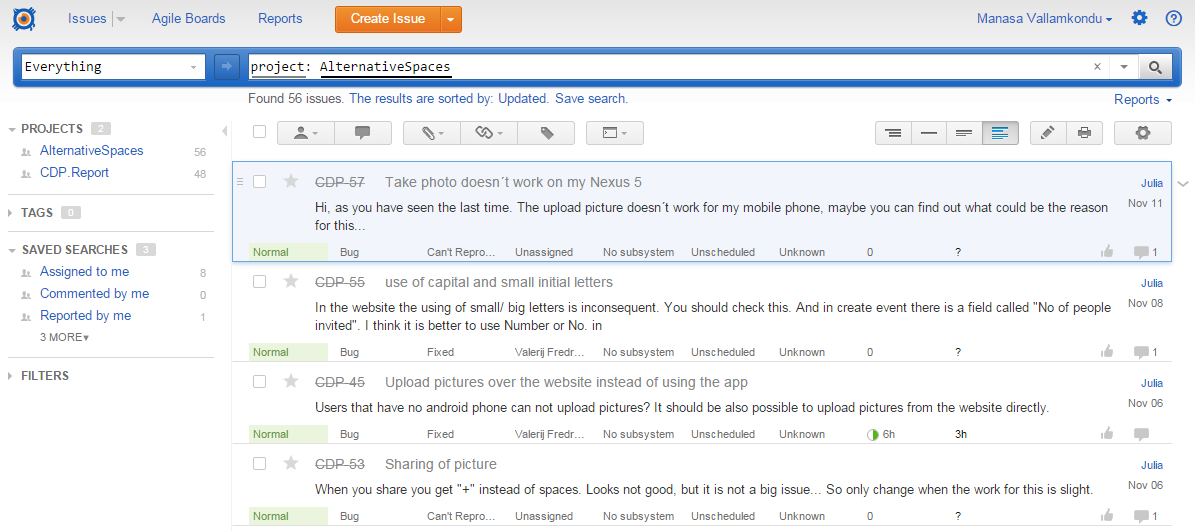
\includegraphics[width=\linewidth]{./Planning/img/YouTrackPage}
  \caption{Browser page for issues in ASpaces from YouTrack.}
  \label{fig:PlanningSoftwareDevYouTrack}
\end{figure}